%!TEX program = xelatex
\documentclass[11pt]{article}

\usepackage[x11names]{xcolor} % needed to declare before tikz
\usepackage{amsmath,  latexsym, amssymb, url, amssymb, pgfplots, amsthm, mathtools, setspace, commath, tikz, verbatim, array, enumitem, bbding, bigints, fontspec, xunicode, xltxtra, geometry, algorithm, algpseudocode, graphicx,listings,lipsum,tabto,tcolorbox,sectsty,booktabs,siunitx,caption, float}
\usepackage[version=4]{mhchem}
\usepackage[utf8]{inputenc}

\NumTabs{6}

\defaultfontfeatures{Mapping=tex-text} 

\setmainfont{Charter} 

\newfontfamily\Codefont{Courier}  %{GillSans} %{AmericanTypewriter}

\definecolor{gry}{rgb}{.95,.95,.95}

\lstset{language=C++,
                moredelim=[is][\color{Green3}\Codefont]{<}{>},
                basicstyle=\small\Codefont,
                identifierstyle=\Codefont,
                directivestyle=\color{Coral1}\Codefont,
                keywordstyle=\color{DeepPink2}\Codefont,
                stringstyle=\color{SeaGreen4}\Codefont,
                commentstyle=\color{Snow4}\Codefont,
                emphstyle=\color{DeepSkyBlue3}\Codefont,
                emph={double,int,float,void,long},
                showspaces=false,
                %keywordstyle=[2]\color{Violet},
                keywords=[2]{*,1,2,3,4,5,6,7,8,9,0},
                keywordstyle=[2]\color{blue},
                showstringspaces=false,
                morecomment=[l][\color{orange}]{\#}}
\lstset{literate=%
    *{0}{{{\color{DarkOrchid3}0}}}1
    {1}{{{\color{DarkOrchid3}1}}}1
    {2}{{{\color{DarkOrchid3}2}}}1
    {3}{{{\color{DarkOrchid3}3}}}1
    {4}{{{\color{DarkOrchid3}4}}}1
    {5}{{{\color{DarkOrchid3}5}}}1
    {6}{{{\color{DarkOrchid3}6}}}1
    {7}{{{\color{DarkOrchid3}7}}}1
    {8}{{{\color{DarkOrchid3}8}}}1
    {9}{{{\color{DarkOrchid3}9}}}1
    {.0}{{{\color{DarkOrchid3}.0}}}2
    {.1}{{{\color{DarkOrchid3}.1}}}2
    {.2}{{{\color{DarkOrchid3}.2}}}2
    {.3}{{{\color{DarkOrchid3}.3}}}2
    {.4}{{{\color{DarkOrchid3}.4}}}2
    {.5}{{{\color{DarkOrchid3}.5}}}2
    {.6}{{{\color{DarkOrchid3}.6}}}2
    {.7}{{{\color{DarkOrchid3}.7}}}2
    {.8}{{{\color{DarkOrchid3}.8}}}2
    {.9}{{{\color{DarkOrchid3}.9}}}2
}
\lstset{alsolanguage=[90]Fortran}
\lstset{alsolanguage=python}
\lstset{backgroundcolor=\color{gry}}
\lstset{frame=single}
\lstset{
    numbers=left,
    numberstyle=\Codefont,
    title=\lstname,
    tabsize=4,
}
\geometry{margin=1in}
\geometry{letterpaper} % or letterpaper (US) or a5paper or....
\usepackage[parfill]{parskip} % Activated to begin paragraphs with an empty line rather than an indent

\title{PHY 480 - Computational Physics \\ Modeling the Solar System}
\author{Thomas Bolden}
\date{April 4, 2016}

\usepackage{hyperref}
\hypersetup{
    colorlinks=true,
    linkcolor=darkgray,
    filecolor=magenta,      
    urlcolor=Aquamarine3, %DarkSlateGray4,
}

\setcounter{secnumdepth}{0} % deactivate for section numbers
%\sectionfont{\fontsize{12}{15}\selectfont} % Activate for same font size sections
\subsectionfont{\fontsize{15}{15}\selectfont}
\newenvironment{amatrix}[1]{%
  \left[\begin{array}{@{}*{#1}{c}|c@{}}
}{%
  \end{array}\right]
}

\setmainfont{Charter}

% =================================================================

\begin{document}

\maketitle

\thispagestyle{empty}

\centerline{Github Repository at \href{https://github.com/ThomasBolden/PHY-480-Spring-2016}{https://github.com/ThomasBolden/PHY-480-Spring-2016}}

\begin{abstract}

    \lipsum[1-1]

\end{abstract}

\vfill

\tableofcontents

\vspace{3cm}

\pagebreak

\subsection{Introduction}

    . 

    In this project, ...

\subsection{Methods}

    %\begin{algorithm}
    %\caption{Verlet Velocity}
    %\label{Verlet Velocity}
    %\begin{algorithmic}[1]
    %\Function{GaussElim}{A}
    %\For{$k=1$ to  $n-1$}
    %\For{$i=k+1$ to $n$}
    %\State $a_{ik} = \frac{a_{ik}}{a_{kk}}$
    %\For{$j=k+1$ to $n+1$}
    %\State $a_{ij}=a_{ij}-a_{ik}\times a_{kj}$
    %\EndFor
    %\EndFor
    %\EndFor
    %\EndFunction
    %\end{algorithmic}
    %\end{algorithm}

    %\begin{algorithm}
    %\caption{Runge-Kutta 4}
    %\label{Runge-Kutta 4}
    %\begin{algorithmic}[1]
    %\Function{GaussElim}{A}
    %\For{$k=1$ to  $n-1$}
    %\For{$i=k+1$ to $n$}
    %\State $a_{ik} = \frac{a_{ik}}{a_{kk}}$
    %\For{$j=k+1$ to $n+1$}
    %\State $a_{ij}=a_{ij}-a_{ik}\times a_{kj}$
    %\EndFor
    %\EndFor
    %\EndFor
    %\EndFunction
    %\end{algorithmic}
    %\end{algorithm}

    . 

\subsection{Results}

    .

    %\begin{table}[H]
    %\caption{Checking $\rho$ Dependency for Various Matrix Dimensionality}
    %\[
    %\begin{array}{cc}
    %\toprule \midrule
    % \text{Minimum } \rho_\text{max} & \text{Matrix Dimensions } n  \\ \midrule
    %5 & 200 \\ \midrule
    %6 & 250 \\ \midrule
    %7 & 300 \\ \midrule
    %8 & 350 \\ \midrule
    %9 & 400 \\ \midrule
    %10 & 450 \\ \midrule
    %\bottomrule
    %\end{array}
    %\]
    %\end{table}

    %\begin{figure}[H] \begin{center}
    %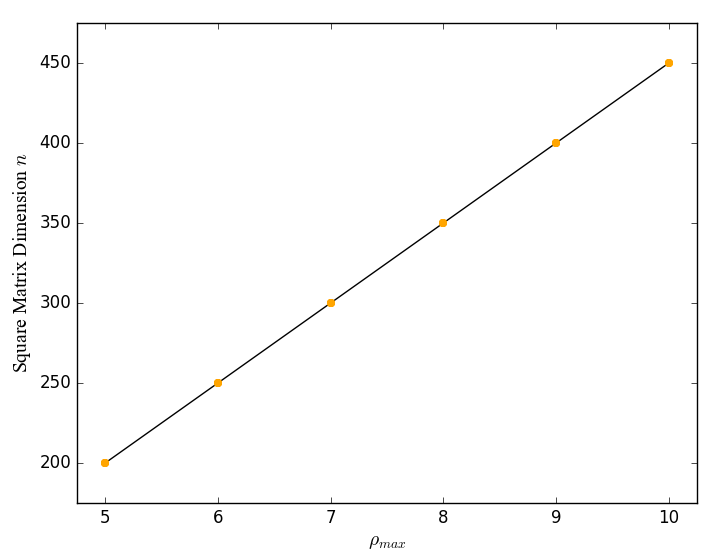
\includegraphics[width=0.8\textwidth]{../Code/RhoDepend.png}
    %\end{center} \caption{Value of $\rho$ Required for Accurate Eigenvalues} \end{figure}

    .

    %\begin{figure}[H] \begin{center}
    %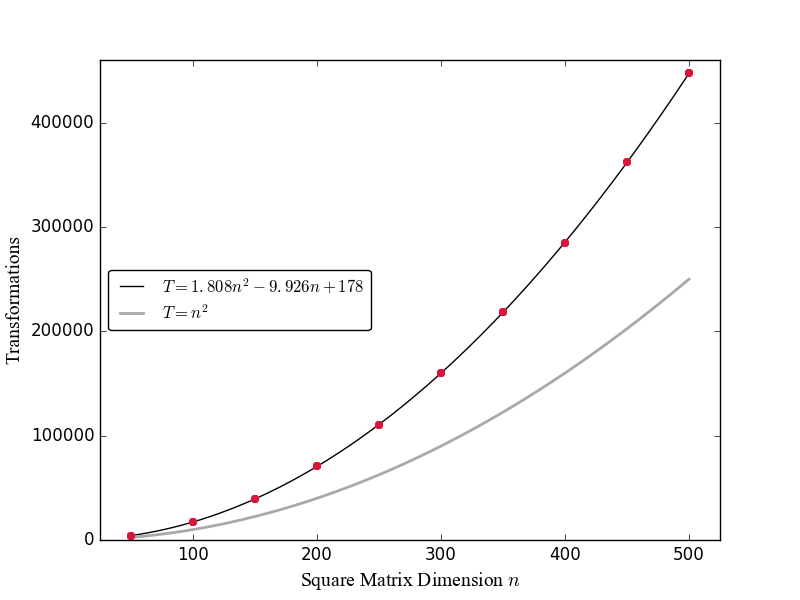
\includegraphics[width=0.6\textwidth]{../Code/TvsN.png}
    %\end{center} \caption{Tansformations Increasing with Dimensionality} \end{figure}

\subsection{Conclusions}

    The first task was to.

\subsection{Code}

    %\lstinputlisting[language=C++]{../Code/EigensolverTests.cpp}

\begin{thebibliography}{1}

\bibitem{morten} 
    M. Hjorth-Jensen, {\em Computational Physics}, University of Oslo (2015). 

\end{thebibliography}

\end{document}
















